\documentclass[12pt, a4paper]{article}

\usepackage{graphicx}
\usepackage{float}
\usepackage{hyperref}

\hypersetup{
	colorlinks=true,
	linkcolor=black
}


\begin{document}
	\pagenumbering{gobble}
	\begin{titlepage}
		\makebox[\textwidth]{\large  Department of Electrical and Electronic Engineering}
		\vspace*{1.5cm}
		\makebox[\textwidth]{\large University of Johannesburg}
		\makebox[\textwidth]{\textbf{EEP3B21 2018}}
		\vspace*{1.5cm}
		\makebox[\textwidth]{\textit{Lecturer: Dr. AR Ndjiongue}}
		\makebox[\textwidth][l]{\large ELECTRONICS}
		\vspace*{1.5cm}
		\makebox[\textwidth][r]{\large Group Project}
		\vspace*{0.5cm}
		\makebox[\textwidth]{\LARGE Group Project 2 Report}
		\vspace*{0.1cm}
		\makebox[\textwidth]{\large Ruan de Bruyn - 216054484}
		\vspace*{0.1cm}
		\makebox[\textwidth]{\large Quintin Kruger - 216054484}
		\vspace*{0.1cm}
		\makebox[\textwidth]{\large Wesley Richardson - 216054484}
		\vspace*{0.3cm}
		\makebox[\textwidth]{\today}
		\vfill
		\noindent I hereby declare that, except where specifically indicated, the work submitted herein is my own original work\\
		Signed: \hspace*{5cm} Date:
	\end{titlepage}

	\pagenumbering{roman}
	\tableofcontents
	\newpage
	\pagenumbering{arabic}

\section{Theoretical Background}

	\subsection{Modulator}
		Amplitude modulation is the simplest modulation technique. A high frequency signal is modulated to carry a lower frequency signal (the lower frequency signal cannot be transmitted effectively as the antenna required to receive a signal with a low frequency is required to be long in lenght - he length of the antenna is inversely proportional to the frequency it is to receive).

		The high frequency signal is knwon as the carrier signal while the signal that needs to be transmitted is called the message signal. 

		To implement a modulator circuit, consider the 3 components that need to be made up by the circuit:
		\begin{enumerate}
			\item Carrier frequency generator
			\item Message frequency generator
			\item AM modulator
		\end{enumerate}

		The modulator circuit used for this experiment is shown in the figure 
		\begin{figure}
			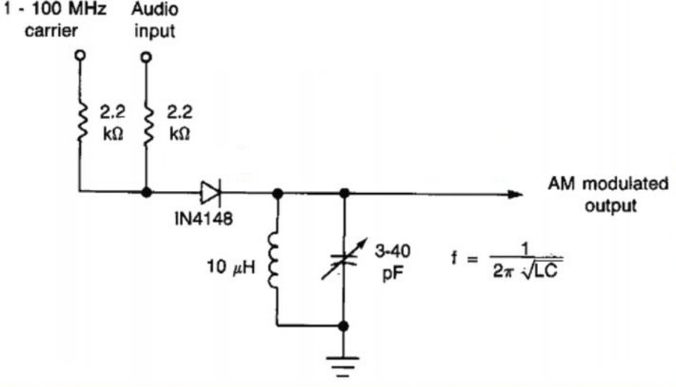
\includegraphics{images/modulator_circuit.png}
			\label{fig:modulator_circuit}
			\caption{The circuit used to implement the modulator.}
		\end{figure}

		The figure shows a frequency equation given as $\frac{1}{2\pi\sqrt{LC}}$. This equation is used to find the value of the capacitor for the modulator circuit (as shown in Figure \ref{fig:modulator_circuit}).
	\subsection{Demodulator Circuit}
		A demodulator circuit is one of the applications of a diode as a detector for amplitude modulated (AM) radio signals. An AM signal consists of a radio-frequency carrier wave whose amplitude varies with different audio frequencies.

		The detector circuit circuit is essentially a half-wave rectifier circuit with an RC filter placed on the output as can be seen from the circuit of the modulator circuit for this practical in Figure \ref{demodulator_circuit}.

		The RC time constant of the filter should fall between 2 values
		\begin{equation}
			\frac{1}{\omega_c} \le RC \le \frac{\sqrt{1-\mu^2}}{\omega_m\mu}
		\end{equation}

		where $\omega_c$ is the frequency of the carrier, $\omega_m$ is the angular frequency of the information and $\mu$ is the modulation index

		This result comes from practical experience in the field of electronic engineering rather than from a mathematical principles.

		If the $RC$ time constant is too small, there would be ripples of the carrier frequency on the output (this is to be avoided as we require the information sent rather than the distortion thereof with the carrier signal).

		If the $RC$ time constant is too big, it will significantly attenuate high frequencies 


		\begin{figure}[H]
			\centering
			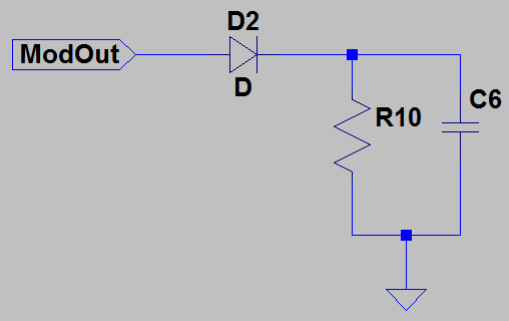
\includegraphics[width=0.7\textwidth]{images/Demodulator_circuit.png}
			\caption{The demodulator circuit used for this experiment}
			\label{fig:demodulator_circuit}
		\end{figure}

	\subsection{}

\section{Experimental Method} % (fold)
\label{sec:experimental_method}

	
% section experimental_method (end)

\section{Results} % (fold)
\label{sec:results}
	\begin{figure}[H]
		\label{fig:carrier}
		\centering
		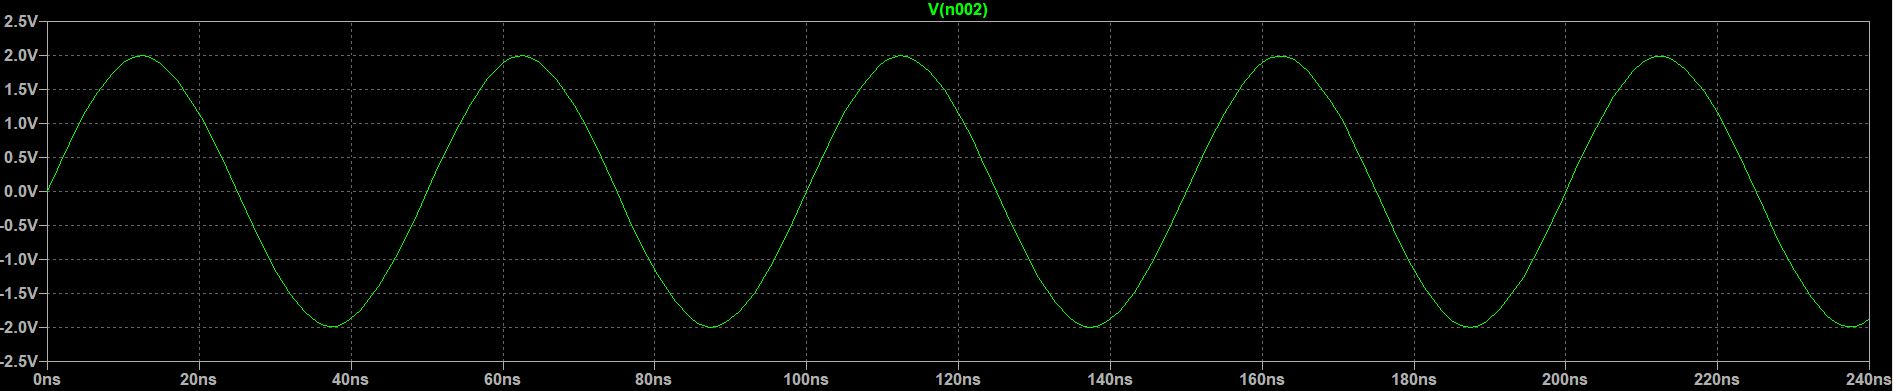
\includegraphics[width=.8\textwidth]{images/carrier.JPG}
		\caption{20 MHz Carrier signal}
	\end{figure}

	\begin{figure}[H]
		\label{fig:modulating}
		\centering
		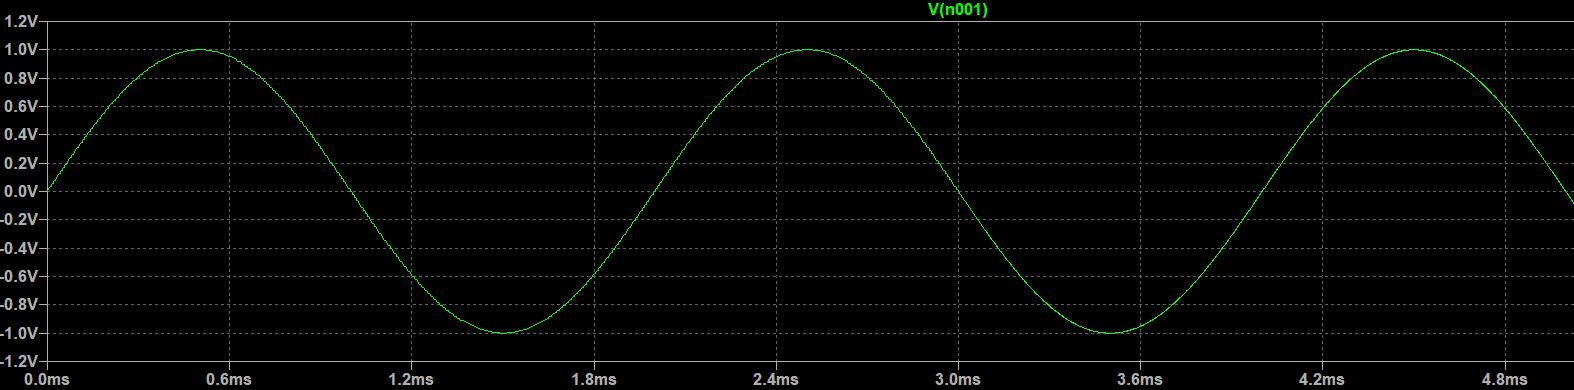
\includegraphics[width=.8\textwidth]{images/modulating.JPG}
		\caption{500 Hz input signal}
	\end{figure}

	\begin{figure}[H]
		\label{fig:output_modulated}
		\centering
		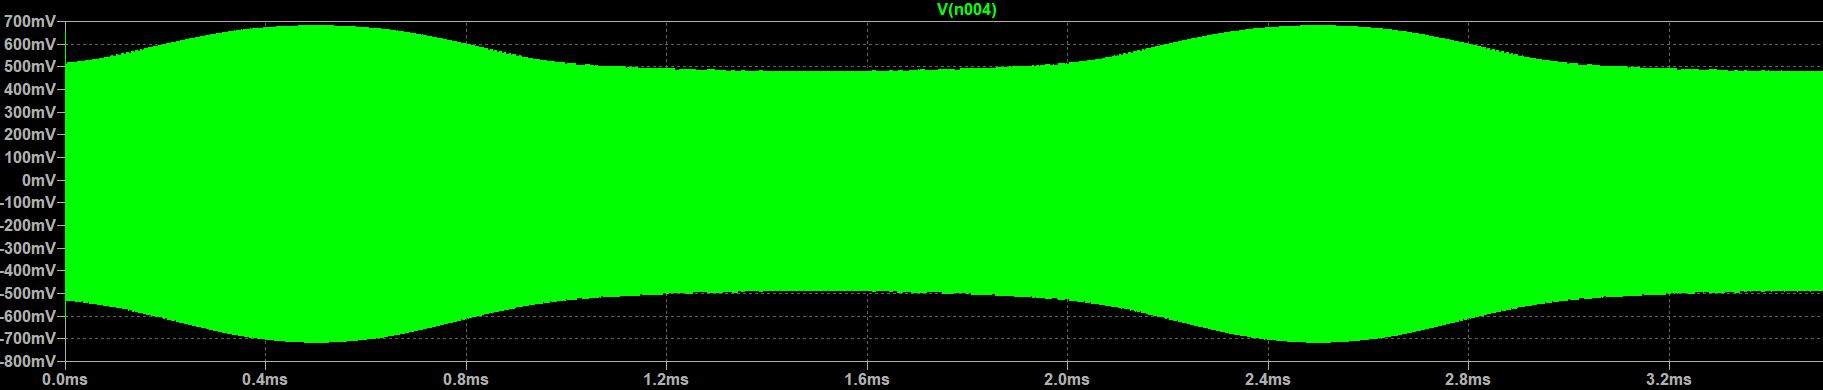
\includegraphics[width=.8\textwidth]{images/output_modulated.JPG}
		\caption{Modulator output}
	\end{figure}

	\begin{figure}[H]
		\label{fig:output_demodulated}
		\centering
		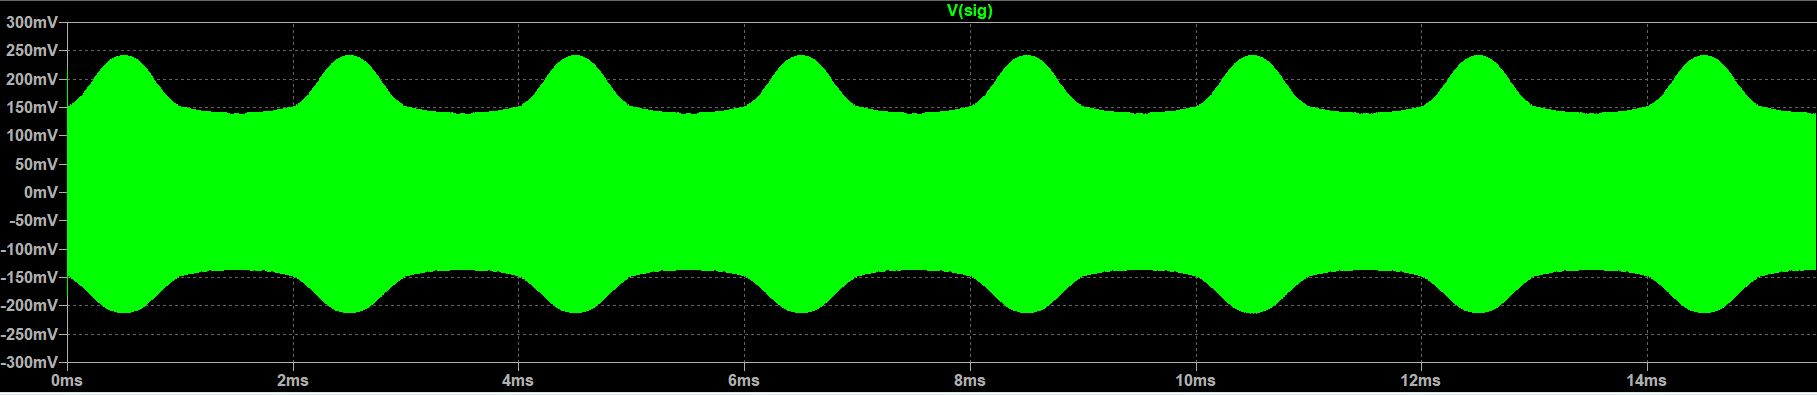
\includegraphics[width=.8\textwidth]{images/output_demodulated.JPG}
		\caption{Demodulated output}
	\end{figure}
% section results (end)

\section{Discussion} % (fold)
\label{sec:discussion}
	In this practical, we have chosen the carrier wave with a frequency of 50 MHz, and an amplitude of 5V. In order to simulate audio input, we simply chose a signal generator which generates a 500 Hz sine wave at an amplitude of 1V. 
% section discussion (end)

\section{Conclusion} % (fold)
\label{sec:conclusion}
	
% section conclusion (end)

\begin{thebibliography}{500}

	\bibitem{lamport94}
	  Donald A. Neamen,
	  \textit{Microelectronics: Circuit Analysis and Design}

	\bibitem{Detector}
	Phil Frost
	\textit{RC time constant and diode detector}
	\texttt{https://electronics.stackexchange.com/questions/100518/rc-time-constant-and-diode-detector}

\end{thebibliography}

\end{document}